\documentclass{article}
\usepackage[utf8]{inputenc}
\usepackage{amsmath, amssymb, tikz, graphics, biblatex, geometry, enumitem, float}
\DeclareMathOperator{\pro}{Proj}
\setlength{\parskip}{1em}
\setlength{\parindent}{0em}

\newcommand{\grstep}[2][\relax]{%
   \ensuremath{\mathrel{
       {\mathop{\longrightarrow}\limits^{#2\mathstrut}_{
                                     \begin{subarray}{l} #1 \end{subarray}}}}}}
\newcommand{\swap}{\leftrightarrow}

\usepackage{pgf,tikz,pgfplots}
\pgfplotsset{compat=1.15}
\usepackage{mathrsfs}
\usetikzlibrary{arrows}
\pagestyle{empty}
\definecolor{qqqqff}{rgb}{0,0,1}
\definecolor{qqwuqq}{rgb}{0,0.39215686274509803,0}

\title{MA2101 19/20 Sem 1}
\author{Yip Jung Hon A0199560R}

\usepackage{lipsum}

\begin{document}
\maketitle
\subsection*{Question 1}
\begin{enumerate}[label=(\alph*)]
    \item The inverse is $\frac{a-bi}{a^2+b^2}$. Easily checked by multiplying by $a+bi$.
    \item We have:
    \begin{equation*}
        \left(\begin{array}{rr|r}
    i + 1 & i + 1 & i \\
    2 i + 1 & i & 2
    \end{array}\right)  \grstep[]{RREF} \left(\begin{array}{rr|r}
    1 & 0 & 1 \\
    0 & 1 & 2 i + 1
    \end{array}\right)
        \end{equation*}
\end{enumerate}

\subsection*{Question 2}
\begin{enumerate}[label=(\alph*)]
    \item Define $E_1, E_2, E_3$ to be the 3 basis matrices given in $E$.

One has, $[T_A(E_1)]_E = 
    \begin{bmatrix} 
    0 \\
    -2b \\
    2c
    \end{bmatrix}$, $[T_A(E_2)]_E = 
    \begin{bmatrix} 
    -c \\
    2a \\
    0
    \end{bmatrix}$ and $[T_A(E_3)]_E = 
    \begin{bmatrix} 
    b \\
    0 \\
    -2a
    \end{bmatrix}$. 
    
    So $[T_A]_{EE}=
    \begin{bmatrix} 
    0 & -c & b\\
    -2b & 2a & 0\\
    2c & 0 & -2a
    \end{bmatrix}$
    \item We have that $[T_A]_{E}=\left(\begin{array}{rrr}
    0 & -c & b \\
    -2 \, b & 2 \, a & 0 \\
    2 \, c & 0 & -2 \, a
    \end{array}\right) \grstep[]{RREF} \left(\begin{array}{rrr}
    1 & 0 & -a/c \\
    0 & 1 & -b/c \\
    0 & 0 & 0
    \end{array}\right)$.
    Since the matrix has a zero row, the kernel is non-trivial.
    \item Note that the characteristic polynomial for $A$ is $c_A(x)=\det\begin{bmatrix} 
    a-\lambda & b \\
    c & -a-\lambda
    \end{bmatrix}=\lambda^2 - (a^2+bc)$
    On the other hand, the characteristic polynomial for $T$ is
    
    $c_T(x)=\det\begin{bmatrix} 
    -\lambda & -c & b\\
    -2b & 2a-\lambda& 0\\
    2c & 0 & -2a-\lambda
    \end{bmatrix}=4a^2\lambda + 4bc\lambda - \lambda^3=\lambda(4a^2+4bc-\lambda^2)$.
    
    Suppose $A$ is diagonalizable. If $a^2+bc \neq 0$, one has that $A$ is diagonalizable since $c_A(x)$ has 2 distinct roots. But this would also mean $4a^2+4bc \neq 0$ and so $\lambda =0$ is not a root for $4a^2+4bc-\lambda^2$. This would imply $c_T(x)$ has 3 distinct roots and hence $T$ is diagonalizable. 
    
    If $a^2+bc=0$, $A$ being diagonalizable implies the dimension of the eigenspace associated to $0$ is 2. That is $\dim(E_0)=2$. This implies $A$ is the zero operator, $a=b=c=0$, and hence $[T_A]_{EE}$ is the zero operator as well, and it is trivially diagonalizable.
    
    Now suppose $T$ is diagonalizable. If $a^2+bc \neq 0$, one has $\sqrt{a^2+bc}, -\sqrt{a^2+bc}$ being 2 distinct roots for $c_A(x)$, implying that $A$ is diagonalizable.
    
    Lastly, if $a^2+bc= 0$ and $T$ is diagonalizable, it means $\dim(E_0)=3$ and $T$ is the zero operator. This means $a=b=c=0$ and $A$ is the zero operator and hence is diagonalizable as well.
\end{enumerate}

\subsection*{Question 3}
\begin{enumerate}[label=(\alph*)]
    \item Let $B=\{M_{11}, M_{12}, M_{21}, M_{22}\}$ be the standard basis for $\mathcal{M}_{2 \times 2} \mathbb{(C)}$.

$T(M_{11})=\begin{bmatrix} 
    1\\
    1 \\
    -1 \\
    0
    \end{bmatrix}$, $T(M_{12})=\begin{bmatrix} 
    \ 0\ \\
    \ 0\  \\
    \ 0\  \\
    \ 0\ 
    \end{bmatrix}$, $T(M_{21})=\begin{bmatrix} 
    1\\
    1 \\
    -1 \\
    0
    \end{bmatrix}$, $T(M_{22})=\begin{bmatrix} 
    1\\
    0 \\
    -1 \\
    0
    \end{bmatrix}$
    
    One has: $T=\begin{bmatrix} 
    1 & 0 & 1 & 1\\
    1 & 0 & 1 & 0\\
    -1 & 0 & -1 & -1 \\
    0 & 0 & 0 & 0
    \end{bmatrix}$, $T-\lambda I=\begin{bmatrix} 
    1-\lambda & 0 & 1 & 1\\
    1 & -\lambda & 1 & 0\\
    -1 & 0 & -1-\lambda & -1 \\
    0 & 0 & 0 & -\lambda
    \end{bmatrix}$. 
    
    Then $\det(T-\lambda I)=\lambda^4$, and the eigenvalues are simply $0$.
    \item For $\ker(T)$, 
    \begin{equation*}
    \begin{bmatrix} 
        1 & 0 & 1 & 1\\
        1 & 0 & 1 & 0\\
        -1 & 0 & -1 & -1 \\
        0 & 0 & 0 & 0
        \end{bmatrix} \grstep[]{RREF} \begin{bmatrix} 
        1 & 0 & 1 & 0 \\
        0 & 0 & 0 & 1 \\
        0 & 0 & 0 & 0 \\
        0 & 0 & 0 & 0
        \end{bmatrix}
    \end{equation*}
        
    So $\ker(T)=\text{span}\{[(0,1,0,0)]_B, [(-1,0,1,0)]_B\}=\text{span}\Bigg\{\left[\begin{array}{rr}
    0 & 1 \\
    0 & 0
    \end{array}\right], \left[\begin{array}{rr}
    -1 & 0 \\
    1 & 0
    \end{array}\right]\Bigg\}.$ 
    \item  We know $m_T(x) \mid c_T(x)$, so it is either $x, x^2, x^3$ or $x^4$. By brute force, it is $x^2$.
    \item Since the minimal polynomial is of degree 2, we know the largest size of the Jordan block is of size 2. 
    
    Let $\{v_1, v_2, v_3, v_4\}$ be an ordered basis for $V$. We set $v_1=[(0,1,0,0)]_B$ and $v_3=[(-1,0,1,0)]_B$. In order to get $T$ in Jordan Canonical Form, we need to find $v_2$ and $v_4$ such that $T(v_2)=v_1$ and $T(v_4)=v_3$. We want to solve:
    \begin{equation*}
        \left[\begin{array}{rrrr|r}
    1 & 0 & 1 & 1 & 0 \\
    1 & 0 & 1 & 0 & 1 \\
    -1 & 0 & -1 & -1 & 0 \\
    0 & 0 & 0 & 0 & 0
    \end{array}\right] \grstep[]{RREF} \left[\begin{array}{rrrr|r}
    1 & 0 & 1 & 0 & 1 \\
    0 & 0 & 0 & 1 & -1 \\
    0 & 0 & 0 & 0 & 0 \\
    0 & 0 & 0 & 0 & 0
    \end{array}\right] 
    \end{equation*}
    Any vector that satisfies this equation will work. We can pick $v_2=[(1,0,0-1)]_B$.
    
    Similar, one can solve:
    \begin{equation*}
        \left[\begin{array}{rrrr|r}
    1 & 0 & 1 & 1 & -1 \\
    1 & 0 & 1 & 0 & 0 \\
    -1 & 0 & -1 & -1 & 1 \\
    0 & 0 & 0 & 0 & 0
    \end{array}\right] \grstep[]{RREF} \left[\begin{array}{rrrr|r}
    1 & 0 & 1 & 0 & 0 \\
    0 & 0 & 0 & 1 & -1 \\
    0 & 0 & 0 & 0 & 0 \\
    0 & 0 & 0 & 0 & 0
    \end{array}\right]
    \end{equation*}
    One can pick $v_4=[(0,0,0,-1)]_B$. Then the matrix $P=\left[\begin{array}{rrrr}
    0 & 1 & -1 & 0 \\
    1 & 0 & 0 & 0 \\
    0 & 0 & 1 & 0 \\
    0 & -1 & 0 & -1
    \end{array}\right]$ is the one needed such that $P^{-1}TP=[T]_{B'}$.
    
    Where $B'$ is ordered the basis:
    $\Bigg\{\left[\begin{array}{rr}
    0 & 1 \\
    0 & 0
    \end{array}\right], \left[\begin{array}{rr}
    1 & 0 \\
    0 & -1
    \end{array}\right],
    \left[\begin{array}{rr}
    -1 & 0 \\
    1 & 0
    \end{array}\right],
    \left[\begin{array}{rr}
    0 & 0 \\
    0 & -1
    \end{array}\right]
    \Bigg\}$
    and 
    \begin{equation*}
    [T]_{B'}=\left[\begin{array}{rrrr}
    0 & 1 & 0 & 0 \\
    0 & 0 & 0 & 0 \\
    0 & 0 & 0 & 1 \\
    0 & 0 & 0 & 0
    \end{array}\right]
    \end{equation*}
    is in Jordan form.
\end{enumerate}

\subsection*{Question 4}
\begin{enumerate}[label=(\alph*)]
\item Let $T=\left[\begin{array}{rr}
x & y \\
z & w
\end{array}\right]$, and let $T^* = \left[\begin{array}{rr}
a & b \\
c & d
\end{array}\right]$. Then:

\begin{align*}
    \left \langle \left[\begin{array}{rr}
x & y \\
z & w
\end{array}\right] \left[\begin{array}{r}
u_1  \\
u_2 
\end{array}\right] , \left[\begin{array}{r}
v_1  \\
v_2 
\end{array}\right] \right \rangle &= \left \langle \left[\begin{array}{r}
xu_1 + yu_2 \\
zu_1 + wu_2
\end{array}\right] , \left[\begin{array}{r}
v_1  \\
v_2 
\end{array}\right] \right \rangle \\
&= 4(xu_1 + yu_2) \overline{v_1} + (zu_1+wu_2) \overline{v_2} \\
&= 4xu_1 \overline{v_1} + 4yu_2 \overline{v_1} + zu_1 \overline{v_2} + wu_2 \overline{v_2}
\end{align*}

\begin{align*}
    \left \langle \left[\begin{array}{r}
u_1  \\
u_2 
\end{array}\right] ,  \left[\begin{array}{rr}
a & b \\
c & d
\end{array}\right] \left[\begin{array}{r}
v_1  \\
v_2 
\end{array}\right] \right \rangle &= \left \langle \left[\begin{array}{r}
u_1 \\
u_2
\end{array}\right] , \left[\begin{array}{r}
av_1+bv_2  \\
cv_1+dv_2 
\end{array}\right] \right \rangle \\
&= 4u_1 \overline{(av_1+bv_2} + u_2 \overline{cv_1+dv_2} \\
&= 4\overline{a} u_1 \overline{v_1}+ 4 \overline{b} u_1 \overline{v_2} + u_2 \overline{c} v_1 + u_2 \overline{d} \overline{v_2}
\end{align*}
Since the adjoint is unique if it exists, one has $\overline{a}=x, 4\overline{b}=z, \overline{c}=4y, \overline{d}=w$, and hence:
\begin{align*}
    T^* = \left[\begin{array}{rr}
\overline{x} & \frac{1}{4}\overline{z} \\
4\overline{y} & \overline{w}
\end{array}\right]
\end{align*}
\item For $T$ to be self-adjoint, one needs to have.
\begin{align*}
    T^* = \left[\begin{array}{rr}
\overline{x} & \frac{1}{4}\overline{z} \\
4\overline{y} & \overline{w}
\end{array}\right] = \left[\begin{array}{rr}
x & y \\
z & w
\end{array}\right]
\end{align*}
Since $\overline{x}=x$, $x \in \mathbb{R}$. Similarly, $w \in \mathbb{R}$. $\frac{1}{4}\overline{z}=y$ and $4\overline{y}=z$ gives us $4y=\overline{z}$.
\end{enumerate}
\subsection*{Question 5}
\begin{enumerate}[label=(\alph*)]
\item Let $x \in V_1 \cap V_2$. Then $T(x) \in V_1$, since $V_1$ is $T$-invariant. Similarly, $T(x) \in V_2$. So $T(x) \in V_1 \cap V_2 \implies V_1 \cap V_2$ is $T$-invariant.
\item The operator satisfies the polynomial $x^2+1$, so the minimal polynomial, $m_T(x) \mid x^2+1$. Since $x^2+1$ does not factor (is irreducible) in $\mathbb{R}$, we have $m_T(x)=x^2+1$ as well. $\deg(m_T(x)) = 2 \iff $ the dimension of the cyclic subspace generated by $u$ is 2 for any non-zero $u \in V$. 
\item If $W_u \oplus W_v$ is direct sum, we are done. Otherwise, assume $x \in W_u \cap W_v$. This implies $\dim(W_1) \leq 2, \dim(W_2) \leq 2$. If $\dim(W_u \cap W_v)=2$ we must have $W_u = W_u \cap W_v = W_v$. If $\dim(W_u \cap W_v)=1$, since $W_u \cap W_v=$ is $T$-invariant, $T(x)=\lambda x$ for some $\lambda \in \mathbb{R}$. Further, $T^2(x)=\lambda^2(x)=-x$, which gives $\lambda^2=-1$, which is impossible since all the entries of $T$ are in $\mathbb{R}$ .
\end{enumerate}
\subsection*{Question 6}
\begin{enumerate}[label=(\alph*)]
\item Let's first show that $\{\cos(mx), \sin(mx) \mid 0 \leq m \leq n\}$ is a \textbf{orthogonal basis }first. For any $m,n$, $n \neq m$, 
\begin{align*}
    \langle \cos(mx), \sin(nx) \rangle &= \int_{-\pi}^{\pi} \cos(mx) \sin(nx) dx = 0 
\end{align*}
For any $n,m$,
\begin{align*}
    \langle \cos(nx), \cos(mx) \rangle = \frac{1}{2\pi} \int_{-\pi}^{\pi} \cos(nx) \cos(mx) dx
    = \frac{\delta_{mn}}{2}
\end{align*}
If $m \neq n$, then $\langle \cos(nx), \cos(mx) \rangle=0$. Also,
\begin{align*}
    \langle \sin(mx), \sin(nx) \rangle = \frac{1}{2\pi} \int_{-\pi}^{\pi} \sin(mx) \sin(nx) dx
    = \frac{\delta_{mn}}{2}
\end{align*}
If $m \neq n$, then $\langle \sin(nx), \sin(mx) \rangle=0$.
This shows that it is an orthogonal basis. When $m=n$,$\langle \sin(nx), \sin(nx) \rangle=\frac{1}{2}$, and we can choose our basis to be $\sqrt(2)\sin(nx)$ to normalise the inner product to 1. We may do the same for $\cos(nx)$. We have that our \textbf{orthonormal basis} is:
\begin{equation}
    \mathscr{B}=\{1, \sqrt{2}\sin(mx), \sqrt{2}\sin(mx) \mid 0 \leq m \leq n\}
\end{equation}
\item For the function $f(x)=1+x$, we want to 'project' it onto our $\mathscr{B}$, our orthonormal basis. 
\begin{align*}
    \pro_{\mathscr{B}}(1+x)&= \langle 1+x, 1\rangle(1) + \langle 1+x, \sqrt{2}\sin x  \rangle(\sin x ) + \langle 1+x, \sqrt{2}\cos x  \rangle(\cos x ) + \cdots \\
    &+\langle 1+x, \sqrt{2}\sin(nx)  \rangle(\sin(nx) ) + \langle 1+x, \sqrt{2}\cos(nx)  \rangle(\cos(nx))
\intertext{But for each $\cos(kx)$, $\langle 1+x, \sqrt{2}\cos(kx)\rangle= \frac{1}{2\pi} \int_{-\pi}^{\pi} (1+x) \cos(kx) = \frac{1}{2\pi} \int_{-\pi}^{\pi} \cos(kx) + \frac{1}{2\pi} \int_{-\pi}^{\pi} x\cos(kx)$. $\int_{-\pi}^{\pi} \cos(kx)=0$, and since $\cos(kx)$ is an even function, $x\cos(kx)$ is an odd function and again, $\int_{-\pi}^{\pi} x\cos(kx)=0$. So all the $\langle 1+x, \sqrt{2}\cos(kx)\rangle (\cos(nx))$ vanishes. The sum then reduces to:}
&= 1+ \frac{1}{2\pi} \sqrt{2} \sin x  \int_{-\pi}^{\pi} (1+x) \sqrt{2} \sin(x) dx  +  \cdots \\ 
&+ \frac{1}{2\pi} \sqrt{2} \sin(nx) \int_{-\pi}^{\pi} (1+x) \sqrt{2} \sin(nx) dx 
\intertext{For each $\sin(kx)$, note that $\int_{-\pi}^{\pi} \sin(kx)=0$, since $\sin(kx)$ is a odd function. The sum again reduces.}
&= 1+ \frac{1}{2\pi} \sqrt{2} \sin x  \int_{-\pi}^{\pi} x \sqrt{2} \sin(x) dx  + \cdots +\frac{1}{2\pi} \sqrt{2} \sin(nx)  \int_{-\pi}^{\pi} x \sqrt{2} \sin(nx) dx \\
&= 1 + \frac{1}{\sqrt{2}\pi} \left[ \sum_{k=1}^n \int_{-\pi}^{\pi} x\sin(kx) dx . \sqrt{2} \sin(kx) \right] \\
\intertext{Since $\int_{-\pi}^{\pi} x\sin(kx) dx=\frac{2\pi (-1)^{k+1}}{k}$,}
&= 1 + \frac{1}{\sqrt{2}\pi} \left[ \sum_{k=1}^n \frac{2\pi (-1)^{k+1}}{k} . \sqrt{2} \sin(kx) \right] \\
&= 1+ 2\sum_{k=1}^n \frac{(-1)^{k+1}}{k} \sin(kx)
\end{align*}
This is called the \textbf{Fourier Series Sawtooth Wave}. As a teaser, this is how it the above function approxmiates $f(x)=1+x$ on $[-\pi, \pi]$ for $n=30$:
\begin{figure}[H]
    \centering
    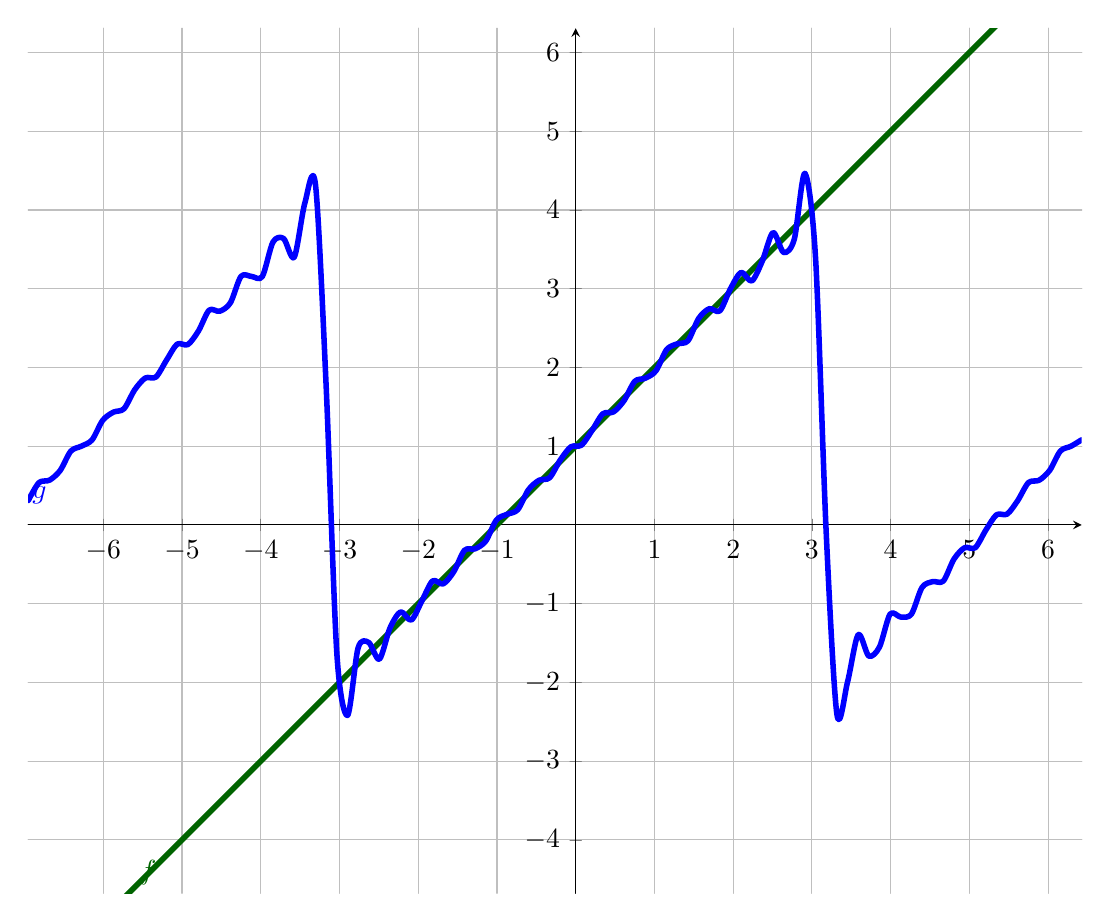
\begin{tikzpicture}[line cap=round,line join=round,>=triangle 45,x=1cm,y=1cm]
\begin{axis}[
x=1cm,y=1cm,
axis lines=middle,
ymajorgrids=true,
xmajorgrids=true,
xmin=-6.952681299116911,
xmax=6.426600129374963,
ymin=-4.677320631353662,
ymax=6.308274190855899,
xtick={-6,-5,...,6},
ytick={-4,-3,...,6},]
\clip(-6.952681299116911,-4.677320631353662) rectangle (6.426600129374963,6.308274190855899);
\draw[line width=2pt,color=qqwuqq,smooth,samples=100,domain=-6.952681299116911:6.426600129374963] plot(\x,{1+(\x)});
\draw[line width=2pt,color=qqqqff,smooth,samples=100,domain=-6.952681299116911:6.426600129374963] plot(\x,{1+2*((-1)^(1+1)/1*sin(((\x))*180/pi)+(-1)^(2+1)/2*sin((2*(\x))*180/pi)+(-1)^(3+1)/3*sin((3*(\x))*180/pi)+(-1)^(4+1)/4*sin((4*(\x))*180/pi)+(-1)^(5+1)/5*sin((5*(\x))*180/pi)+(-1)^(6+1)/6*sin((6*(\x))*180/pi)+(-1)^(7+1)/7*sin((7*(\x))*180/pi)+(-1)^(8+1)/8*sin((8*(\x))*180/pi)+(-1)^(9+1)/9*sin((9*(\x))*180/pi)+(-1)^(10+1)/10*sin((10*(\x))*180/pi)+(-1)^(11+1)/11*sin((11*(\x))*180/pi)+(-1)^(12+1)/12*sin((12*(\x))*180/pi)+(-1)^(13+1)/13*sin((13*(\x))*180/pi)+(-1)^(14+1)/14*sin((14*(\x))*180/pi))});
\begin{scriptsize}
\draw[color=qqwuqq] (-5.430867297771864,-4.415758849872481) node {$f$};
\draw[color=qqqqff] (-6.810011236490813,0.3716143626921475) node {$g$};
\end{scriptsize}
\end{axis}
\end{tikzpicture}
    \caption{Fourier Series Sawtooth Wave}
    \label{fig:my_label}
\end{figure}
\item For any $f,g$ are functions, $d(f,g) = |f-g| = \sqrt{\langle f-g, f-g \rangle}$. Let $f=1+x$ and set $g=1+ 2\sum_{k=1}^n \frac{(-1)^{k+1}}{k} \sin(kx)$.

\begin{align*}
    d\left(f,g \right) &= \left|x-2\sum_{k=1}^n \frac{(-1)^{k+1}}{k} \sin(kx)\right| \\
    &= \sqrt{\frac{1}{2\pi}, \int_{-\pi}^{\pi} \left( x-2\sum_{k=1}^n \frac{(-1)^{k+1}}{k} \sin(kx) \right)^2  } \\
    &= \sqrt{\frac{1}{2\pi} \int_{-\pi}^{\pi} x^2 - 4x \sum_{k=1}^n  \frac{(-1)^{k+1}}{k} \sin(kx) + 4 \left( \sum_{k=1}^n  \frac{(-1)^{k+1}}{k} \sin(kx)) \right)^2 dx }
\intertext{Let's take a closer took at the last term. There's no hope of integrating $ \int_{-\pi}^{\pi}\left( \sum_{k=1}^n  \frac{(-1)^{k+1}}{k} \sin(kx)) \right)^2$ by brute force. However, notice that when you do expand $\left( \sum_{k=1}^n  \frac{(-1)^{k+1}}{k} \sin(kx)) \right)^2$ out, we have a mess of terms of the form $\sin(nx) \sin(mx)$. When the integral $\int_{-\pi}^{\pi}$ acts on each $\sin(nx) \sin(mx)$, if $n \neq m$, the term will go to $0$. The only terms that survive are when $n=m$, that is: $ \int_{-\pi}^{\pi}\left( \sum_{k=1}^n  \frac{(-1)^{k+1}}{k} \sin(kx)) \right)^2 = \int_{-\pi}^{\pi} \sum_{k=1}^n \left(\frac{(-1)^{k+1}}{k} \sin(kx) \right)^2$.}
&= \sqrt{\frac{1}{2\pi} \frac{1}{3} [x^3]^{\pi}_{-\pi} - \frac{4}{2\pi} \sum_{k=1}^n  \frac{(-1)^{k+1}}{k} \int_{-\pi}^{\pi} x\sin(kx) dx + \frac{4}{2\pi} \int_{-\pi}^{\pi} \sum_{k=1}^n \left(\frac{(-1)^{k+1}}{k} \sin(kx) \right)^2 dx } \\
&=\sqrt{\frac{\pi^2}{3} - \frac{4}{2\pi} \sum_{k=1}^n  \frac{(-1)^{k+1}}{k}\frac{(-1)^{k+1}2\pi}{k} + \frac{4}{2\pi} \sum_{k=1}^n \left(\frac{1}{k^2} \int_{-\pi}^{\pi} \sin^2(kx) \right) dx }
\intertext{From (0.3) in the paper, $\int_{-\pi}^{\pi} \sin^2(kx) dx=\pi$.}
&= \sqrt{\frac{\pi^2}{3} - 4 \sum_{k=1}^n  \frac{1}{k^2} + \frac{4}{2\pi} \sum_{k=1}^n \left(\frac{\pi}{k^2} \right) dx } \\
&= \sqrt{\frac{\pi^2}{3} - 2  \sum_{k=1}^n \frac{1}{k^2}}
\end{align*}
Taking $n \to \infty$ gives that $d(f,g) \to 0$, as desired.

\end{enumerate}





\end{document}
